\chapter{Analisi spettrometrica}
\label{ch:spettro}

\section{Setup di acquisizione}
Viene utilizzato lo spettrometro isoplane BES1 (descrizione vedi articolo), con tre diversi grating: 150, 1200 e 2400. Il grating a risoluzione maggiore viene utilizzato per acquisire le righe \ce{OH} e \ce{N_{2,\text{rot}}} (relative agli stati rotazionali), mentre quello a media risoluzione per acquisire le righe \ce{N_{2,\text{vib}}} (relative agli stati vibrazionali). Per acquisire lo spettro totale vengono utilizzati sia il grating a risoluzione minore, sia quello a media risoluzione.

L'apparato sperimentale consiste nella sorgente in funzione a distanza di \SI{1}{\centi\metre} dal bersaglio in metallo (collegato a terra) con l'ottica focalizzata sul flusso di gas, come in foto \ref{fig:app}. Vengono distinte due posizioni dell'ottica, una vicino l'uscita della sorgente, una vicino il punto di impatto sul bersaglio, permettendo di osservare la variazione di intensità delle linee.
I parametri impostati nella sorgente sono quelli del setup standard, $f = \SI{5}{\kilo\hertz}$ e $\Delta t = \SI{16}{\micro\second}$.

\begin{figure}
\centering
\includegraphics[width=.6\textwidth]{Immagini/apparato.jpg}
\caption{Configurazione per le misure spettrometriche. Si vedono la sorgente in funzione, il bersaglio in metallo, obiettivo e fibra ottica a sinistra.}
\label{fig:app}
\end{figure}


Per ogni acquisizione viene stabilito un tempo di acquisizione idoneo ad avere un numero ottimale di eventi, evitando la saturazione dei singoli canali. Una volta stabilito il tempo di acquisizione viene eseguita una misura di fondo, a sorgente spenta, e successivamente viene avviata la misura con sorgente attiva.

\section{Presentazione ed analisi misure}

\subsection{Riconoscimento righe}
Il riconoscimento dei picchi viene effettuato tramite la classe TSpectrum presente nelle librerie ROOT, vengono esclusi i picchi dovuti al fondo.
In figura \ref{fig:spettrotot} si vedono le principali righe estrapolate dalle acquisizioni, in particolare si vedono le righe relative ad \ce{NO}, \ce{OH}, \ce{H_{2}} e \ce{N_{2}}, tabulate in Tabella %\ref{tab:spettrotot}
.

\begin{figure}
\centering
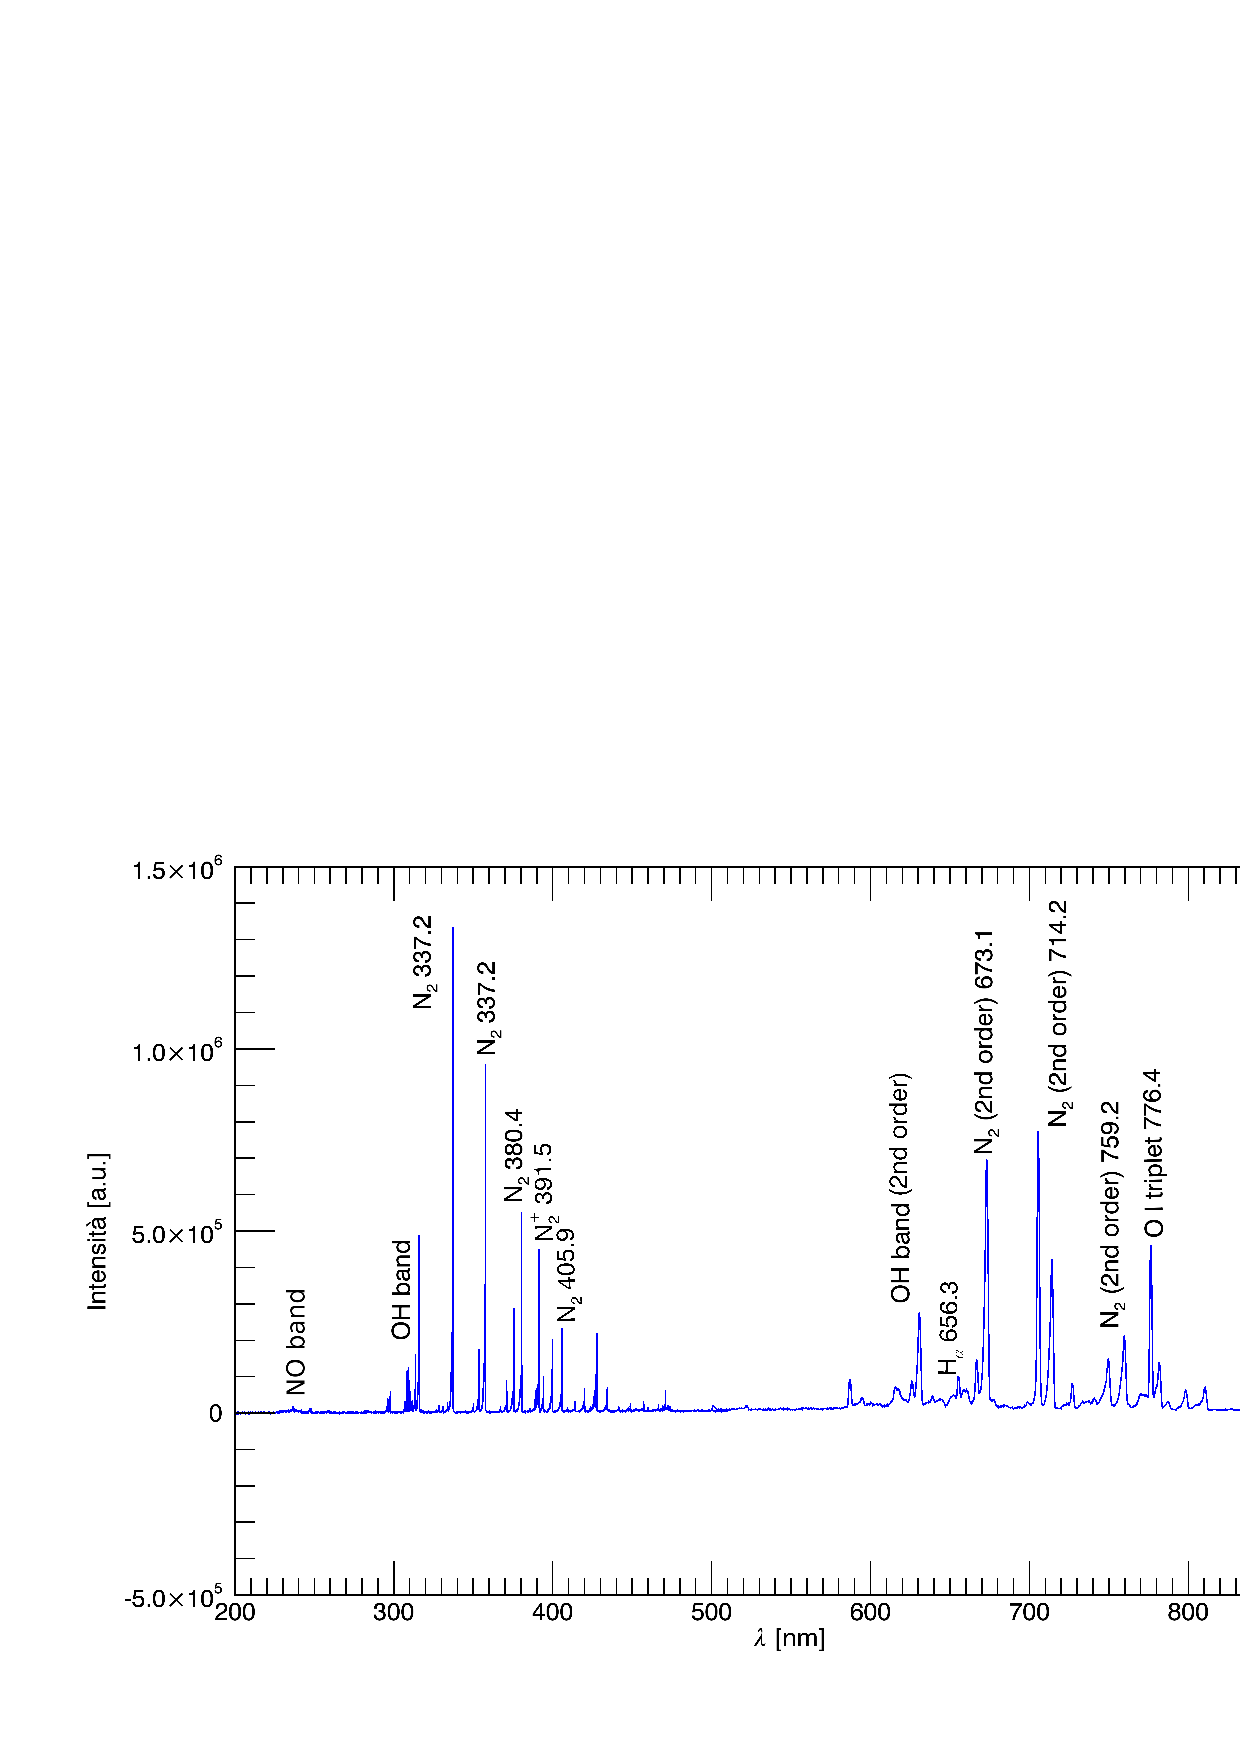
\includegraphics[width=0.99\textwidth]{Immagini/spettrotot_unico_label.png}
\caption{Spettro acquisito con condizioni di misura standard ($f = \SI{5}{\kilo\hertz}$ e $\Delta t = \SI{16}{\micro\second}$), obiettivo puntato vicino l'uscita del gas dalla sorgente.}
\label{fig:app}
\end{figure}

L'acquisizione migliore, nella quale vengono riconosciuti più picchi, è quella mostrata in Figura \ref{fig:spettrotot}, corrispondente alla posizione 1, obiettivo puntato sulla sorgente. L'acquisizione in posizione 2 presenta un rate di conteggi/s molto minore, ma si riescono a riconoscere le transizioni più intense di ogni molecola.


\subsection{\ce{He} + \ce{H_2O} e \ce{He} + \ce{NH_3}}


\subsection{Stima temperatura}
 La procedura consiste nel simulare diversi spettri $S(\lambda,T)$ come presentati in \ref{eq:fitOH} e in \ref{eq:fitN2} e viene selezionato quello dagli scarti minori rispetto le misure.
 
